One of the main tasks of drone flight is simply to hover. Figure \ref{fig:hover_performance} illustrates the performance of the drone in hovering for 30 seconds. It is able to maintain its orientation in the pitch and roll axes quite well, even while changing altitude. The mean and standard deviation for the pitch and roll values during these 30 seconds are shown in Table \ref{tab:attitude}. The included video ``Initial Drone Flights'' provides a more intuitive way to view the stability of the drone's flight performance.\footnote{``Initial Drone Flights'' video: \url{https://vimeo.com/461576798}}

\begin{figure}
    \centering
    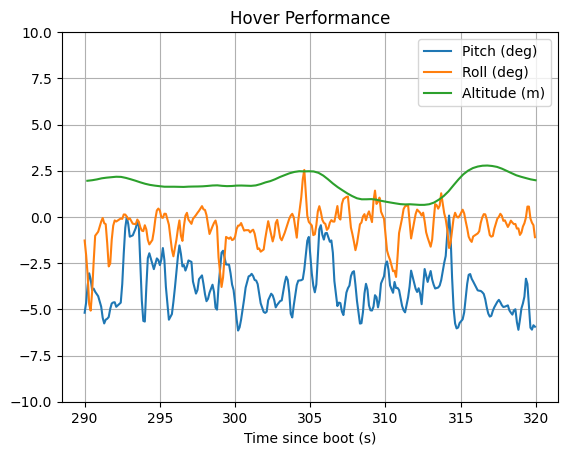
\includegraphics[width=0.7\textwidth]{images/stability.png}
    \caption{Attitude and altitude of the drone during 30 seconds of hovering.}
    \label{fig:hover_performance}
\end{figure}

\begin{table}
    \centering
    \begin{tabular}{|c|c|c|}
    \hline
        \textbf{Data} & \textbf{Mean} & \textbf{Standard Deviation} \\\hline
        Pitch & -3.79\degree & 1.37\degree \\\hline
        Roll & -0.53\degree & 0.98\degree \\\hline
    \end{tabular}
    \caption{Attitude while hovering.}
    \label{tab:attitude}
\end{table}